\section{Ergot's history.}

The presence of rye stains in somewhere's whereabouts foreshadowed one out of two terrible diseases --- almost endemic to some regions. West of the Rhine, patients were bothered by sensations in a limb which, in a few weeks, turned into burning so intense that it was called \enquote{Saint Anthony's fire}. Luckily for the unfortunate, the pain ceased just to be substituted by numbness. The now cold and pale limb blackened, shrank and mummified. The gangrene expanded until finishing with a premature death. On the other side there wasn't much luck either. The sick were attacked by frequent seizures: first fingers, then limbs, hips and finally, the whole body. Covered in vomit they howled in pain, and when it got to the head, the epileptic episodes began as a prelude to blindness, deafness, and death.

Between the 17th and the 18th century, it was discovered that these purple badges were actually the mycelium of a fungus now known as \textit{ergot} (species belonging to the \textit{Claviceps} genus). Furthermore, it was confirmed that the substances this fungus produced directly caused those diseases, and so they were named \textit{ergotism}. Ergot grows parasitically in rye flowers and falls producing fruiting bodies that release ascospores, infecting new grain and repeating the cycle.

Rye isn't new and neither is ergot, and even then we hold no written record of it in Europe until a 16th century herbal, in which its obstetric use (to precipitate labor) is described (Figure \ref{ergotbook}). Almost no other book at the time mentions ergot, so either botanists didn't know about it or didn't consider it relevant. The link between ergot and ergotism generated a stigma against its use as a treatment. Despite having been used by generations of midwives previously, it was forbidden in many european regions. In the New World however, its use was popularised in a boiled powder format (\textit{Pulvis parturiens} or \textit{Pulvis ad partum}) by doctors John Stearns and Akerly. Sold in pharmacies, prescribed by physicians and used by midwives, a cultural transfer to a land free of the prejudices europeans had acquired through centuries of experience was taking place. In 1813, thanks to a very successful dissertation from Oliver Prescott (which was translated and exported to Europe), a general interest on the medicinal properties of this entity arose back. In the 20th century, ergot was produced in tons anually in cities like Vigo, Lisboa and Leningrad. 

\begin{figure}[H]
	\centering

	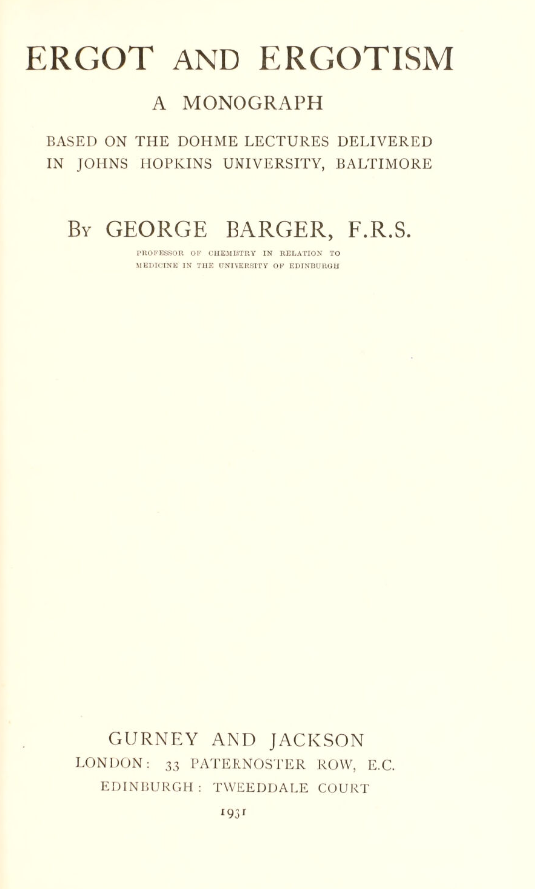
\includegraphics[height=.3\textheight]{media/1-ergotcover.png}
	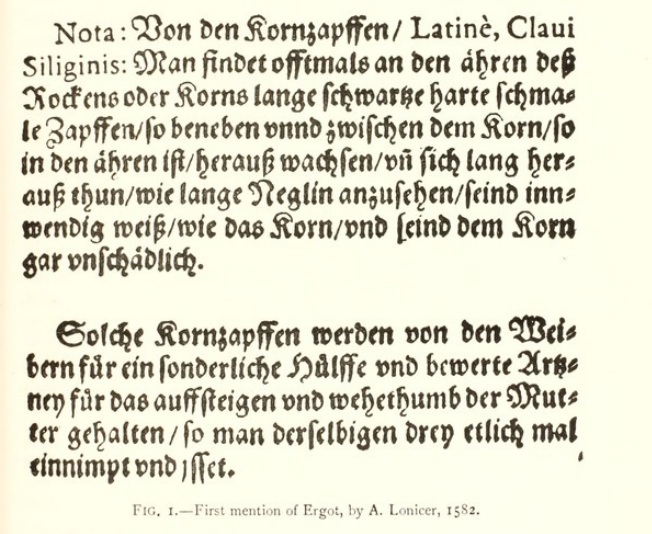
\includegraphics[height=.3\textheight]{media/1-ergotparagraph.png}
	\caption{One of the first written mentions of ergot where its obstetric use is described. The full story of the fungus is exposed to an exquisite detail in the book \textit{Ergot and ergotism}, from which this fragment is taken.}
	\label{ergotbook}
\end{figure}

\subsection{Albert Hofmann's investigations.}

Having come out of the University of Zürich in 1929, chemistry student Albert Hofmann started working in the laboratories of a company named Sandoz. In previous decades, Sandoz had been investigating ergot's alkaloids: substances that, they thought, produced in organisms both the therapeutic and the toxic effects of ergot. If it was achieved to separate the components responsible for uterine contractions from those responsible for ergotism, valuable medicines could be obtained. These studies were leaded by Arthur Stoll, and Albert Hofmann would carry them under his supervision. 

Hofmann made quick progress, isolating the uterotonic and haemostatic components, very useful during labor and which made ergot such a popular remedy in past times; and the common nexus of many ergotic alkaloids: lysergic acid (not to be confused with its diethylamide, LSD. Lysergic acid on its own isn't hallucinogenic) (Figure \ref{alkaloids}).

\begin{figure}[H]
	\centering
	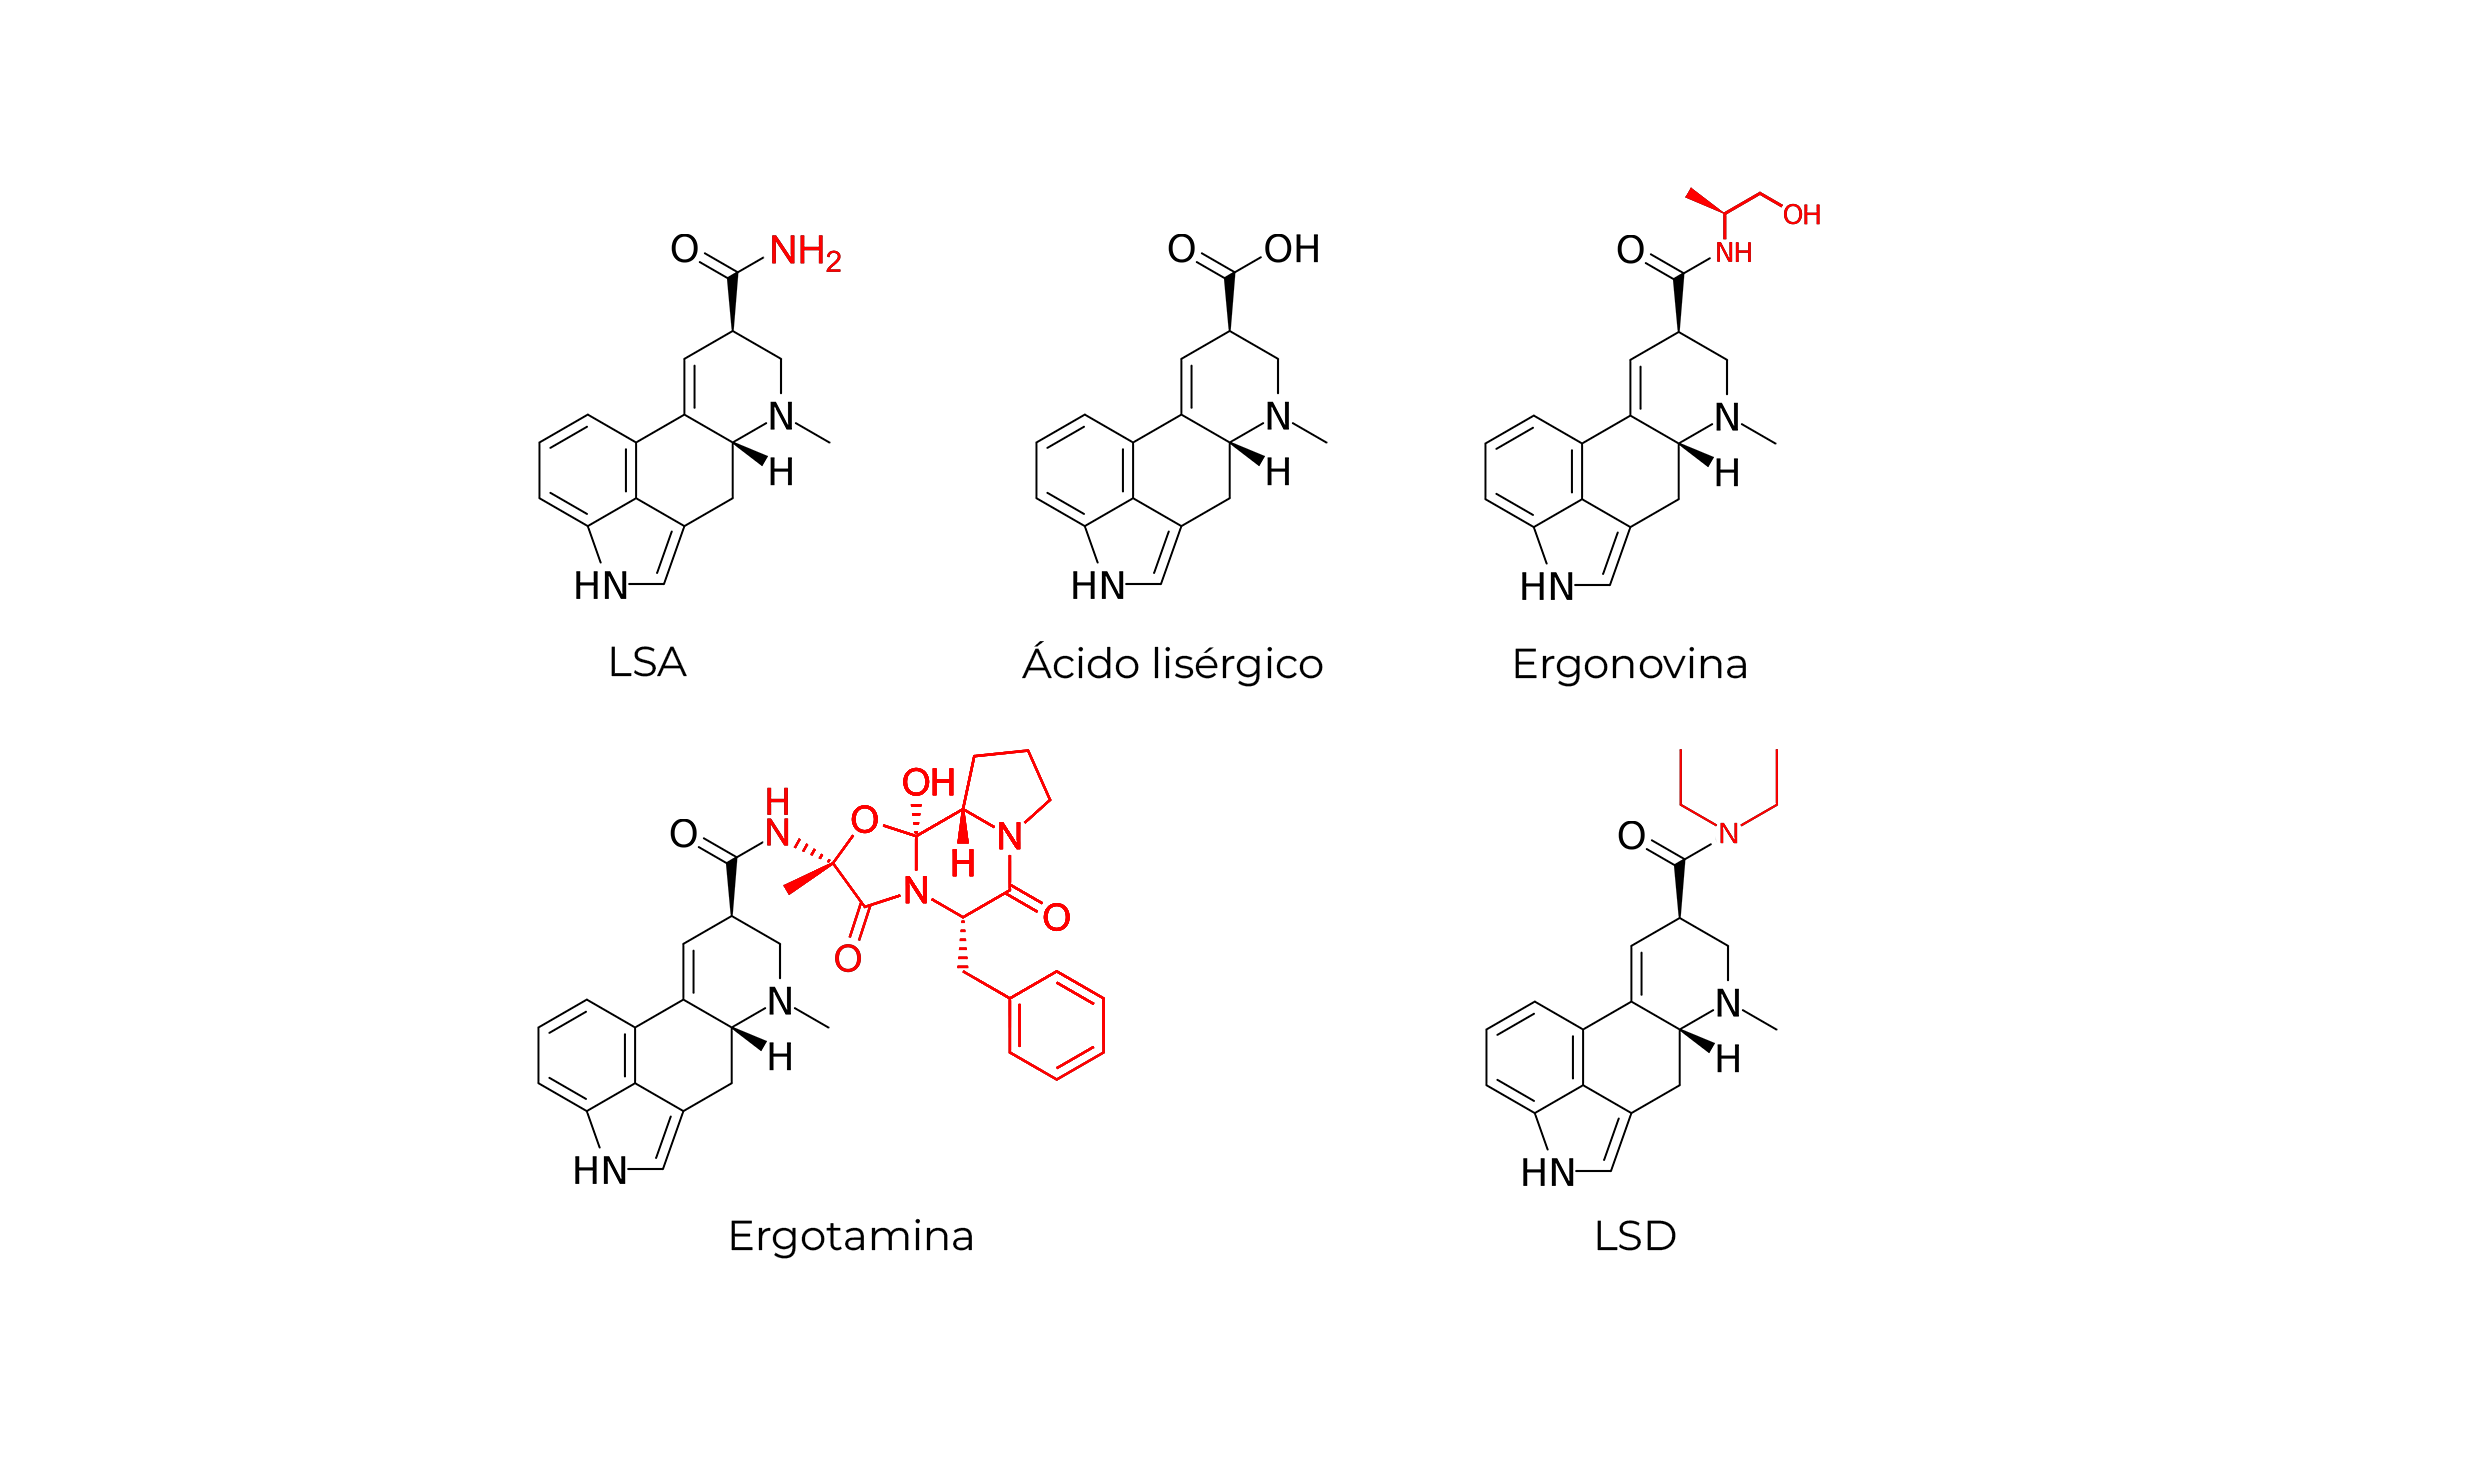
\includegraphics[width=\linewidth]{media/2-alkaloids.png}
	\caption{Many of ergot's alkaloids are derived from lysergic acid (shown in black) through an amide bond to another compound (shown in red). LSD (bottom right) is lysergic acid's di-ethyl-amide, that is, lysergic acid bonded to two ethyl groups through an amide bond.}
	\label{alkaloids}
\end{figure}

Using lysergic acid, Albert Hofmann synthesized dozens of compounds, the twenty-fifth of which was its diethylamide: LSD-25 or simply LSD (\textit{\textbf{L}yserg\textbf{s}äure-\textbf{D}iethylamid}). At first it was considered irrelevant and it wouldn't see the light again until 5 years later, when Hofmann, intrigued by \enquote{the feeling that this substance could possess properties other than those established in the first investigations}, decided to synthesize it again. During the process he suffered a series of strange sensations that he would then report to Stoll:

% Cita
\let\oldquote\quote
\let\endoldquote\endquote
\renewenvironment{quote}[2][]
  {\if\relax\detokenize{#1}\relax
     \def\quoteauthor{#2}%
   \else
     \def\quoteauthor{#2~---~#1}%
   \fi
   \oldquote}
  {\par\nobreak\smallskip\hfill(\quoteauthor)%
   \endoldquote\addvspace{\bigskipamount}}

\begin{quote}[LSD: my problem child]{Albert Hofmann}
	\enquote{Last Friday, April 16,1943, I was forced to interrupt my work in the laboratory in the middle of the afternoon and proceed home, being affected by a remarkable restlessness, combined with a slight dizziness. At home I lay down and sank into a not unpleasant intoxicated-like condition, characterized by an extremely stimulated imagination. In a dreamlike state, with eyes closed (I found the daylight to be unpleasantly glaring), I perceived an uninterrupted stream of fantastic pictures, extraordinary shapes with intense, kaleidoscopic play of colors. After some two hours this condition faded away.}
\end{quote}

He theorized that, in an act of carelessness, a bit of LSD-25 had come into contact with his skin, causing these effects. Were this to be true, the effective dose of this substance would have to be very small. To confirm it, he decided three days later to consume 0.25 miligrams, an amount he considered wise. He felt as if a devil was geting ahold of his mind, body and soul. He feared to be in a transition towards death. He had actually taken two and a half times the dose we now consider standard. Despite that, his physical state was correct (apart from his dilated pupils), so with the passage of time and anxiety, he became able to enjoy the fantastic images that flashed before him. To his surprise, he didn't feel any type of hangover the following day, but rather a sensation of well-being blooming in him. He saw the world as newly made. LSD produces hallucinogenic effects similar to those of mescaline or psilocybin (alkaloids from the \textit{Peyotl} cactus and \textit{Psilocybe} mushrooms respectively) in doses dozens of times smaller and without chronic toxic effects (at those doses). The main danger --- according to Hofmann --- was what could be done or felt during the state of drunkenness. To understand the details of LSD's operation, it's necessary to know in depth what it acts upon.

\newpage
